\documentclass[12pt,a4paper]{article}
%\usepackage{ctex}
\usepackage{amsmath,amscd,amsbsy,amssymb,latexsym,url,bm,amsthm}
\usepackage{epsfig,graphicx,subfigure}
\usepackage{enumitem,balance}
\usepackage{wrapfig}
\usepackage{mathrsfs,euscript}
\usepackage[usenames]{xcolor}
\usepackage[colorlinks,linkcolor = blue]{hyperref}
\usepackage[vlined,ruled,commentsnumbered,linesnumbered]{algorithm2e}

\newtheorem{theorem}{Theorem}
\newtheorem{lemma}[theorem]{Lemma}
\newtheorem{proposition}[theorem]{Proposition}
\newtheorem{corollary}[theorem]{Corollary}
\newtheorem{exercise}{Exercise}
\newtheorem*{solution}{Solution}
\newtheorem{definition}{Definition}
\theoremstyle{definition}
\usepackage{listings}


%
\definecolor{mygreen}{rgb}{0,0.6,0}
\definecolor{mygray}{rgb}{0.5,0.5,0.5}
\definecolor{mymauve}{rgb}{0.58,0,0.82}
\lstset{
	backgroundcolor=\color{white}, 
	basicstyle = \footnotesize,       
	breakatwhitespace = false,        
	breaklines = true,                 
	captionpos = b,                    
	commentstyle = \color{mygreen}\bfseries,
	extendedchars = false,             
	frame =shadowbox, 
	framerule=0.5pt,
	keepspaces=true,
	keywordstyle=\color{blue}\bfseries, % keyword style
	language = C++,                     % the language of code
	otherkeywords={string}, 
	numbers=left, 
	numbersep=5pt,
	numberstyle=\tiny\color{mygray},
	rulecolor=\color{black},         
	showspaces=false,  
	showstringspaces=false, 
	showtabs=false,    
	stepnumber=1,         
	stringstyle=\color{mymauve},        % string literal style
	tabsize=2,          
	title=\lstname                      
}

%\numberwithin{equation}{section}
%\numberwithin{figure}{section}

\renewcommand{\thefootnote}{\fnsymbol{footnote}}

\newcommand{\postscript}[2]
 {\setlength{\epsfxsize}{#2\hsize}
  \centerline{\epsfbox{#1}}}

\renewcommand{\baselinestretch}{1.0}

\setlength{\oddsidemargin}{-0.365in}
\setlength{\evensidemargin}{-0.365in}
\setlength{\topmargin}{-0.3in}
\setlength{\headheight}{0in}
\setlength{\headsep}{0in}
\setlength{\textheight}{10.1in}
\setlength{\textwidth}{7in}
\makeatletter \renewenvironment{proof}[1][Proof] {\par\pushQED{\qed}\normalfont\topsep6\p@\@plus6\p@\relax\trivlist\item[\hskip\labelsep\bfseries#1\@addpunct{.}]\ignorespaces}{\popQED\endtrivlist\@endpefalse} \makeatother
\makeatletter
\renewenvironment{solution}[1][Solution] {\par\pushQED{\qed}\normalfont\topsep6\p@\@plus6\p@\relax\trivlist\item[\hskip\labelsep\bfseries#1\@addpunct{.}]\ignorespaces}{\popQED\endtrivlist\@endpefalse} \makeatother



\begin{document}
\noindent

%========================================================================
\noindent\framebox[\linewidth]{\shortstack[c]{
\Large{\textbf{Lab5  Priority Queues}}\vspace{1mm}\\
VE281 - Data Structures and Algorithms, Xiaofeng Gao, Autumn 2019}}
%VE281 - Data Structures and Algorithms, Xiaofeng Gao, Autumn 2019}}
\begin{center}
	\footnotesize{\color{blue}$*$ Name:Jin Zhejian	\quad Student ID: 517370910167 \quad Email: jinzhejian@outlook.com}
\end{center}




%\section{Motivation}
%\begin{enumerate}
%    \item To give you experience in implementing various sorting algorithms and two linear-time selection algorithms, i.e., random and deterministic selection algorithms.
%    \item To empirically study the run time efficiency of the sort algorithms and two selection algorithms and compare the run time efficiency of the selection algorithms with the sorting algorithms.
%\end{enumerate}
\section{Preparation}
 In order to show the relationship between runtime and grid size better, I choose the grid width 10, 20, 50, 100, 200.  I  generate random numbers and weight (assuming the maximum possible value of weight is 1000) , each grid size for 5 different data in order to calculate the average runtime, and then save them in  .in file. The source code is shown below.
 \begin{lstlisting}[caption={generate.cpp}]
#include <iostream>
#include <fstream>
#include <stdlib.h>

using namespace std;

int main() {
srand((int)time(0));
fstream fso("data_200_1.in", ios::out);
int size = 200;
int weight = 1000;

fso << size << endl;
fso << size << endl;
fso <<  0  << " " << 0 << endl;
fso <<  size-1  << " " << size -1 << endl;
int i;
for (i = 0; i < size*size; ++i)
fso <<  rand()%weight + 1  << ' ';
fso.close();

return 0;
}

 \end{lstlisting}

Then, I calculate the average runtime, the data is shown below:
\begin{table}[ht]
	\begin{center}
	\begin{tabular}{|c|c|c|c|}
		\hline
		size & BINARY & UNSORTED & FIBONACCI \\ \hline
		10   & 179.2  & 254.6    & 232.4     \\ \hline
		20   & 799.4  & 951.4    & 969.2     \\ \hline
		50   & 2540.2 & 3423.6   & 2439.0    \\ \hline
		100  & 5260.4 & 14270.4  & 6680.2    \\ \hline
		200  & 21713  & 108144   & 31526     \\ \hline
	\end{tabular}
	\end{center}
\end{table}


\newpage
\section{Binary Heaps}

In this lab, I implemented 3 heaps, they are: Binary Heap, Unsorted Heap, and Fibonacci Heap. Then, I  use the three heaps I implemented to solve a finding shortest path problem.  I choose the grid width 10, 20, 50, 100, 200, assuming the weight of each point is positive number and doesn't exceed 1000, and I record each of the run times of the 3 heaps for each of the grid size.
 
I  choose clocks as the time of unit.
 
The graph are shown as follows:

\begin{figure}[ht]
	\centering
	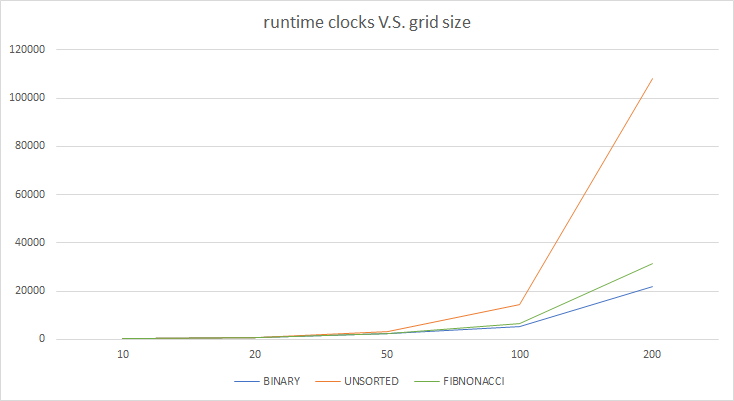
\includegraphics[scale=2.0]{1.png}
	\caption{runtime (clocks) of 3 heaps versus the array size}
\end{figure}

From the figure, we can find that the runtime of Unsorted Heap is slower that of Binary Heap and Fibonacci Heap. However, the run time of  Fibonacci Heap is a little slower than that of Binary Heap, which contradicts to the theoretical knowledge.

Theoretically, the time complexity of \textbf{enqueue} and \textbf{dequeue\_min} of Fibonacci Heap is: $O(1)$ and amortized $O(\log n)$, while 
the time complexity of \textbf{enqueue} and \textbf{dequeue\_min} of Binary Heap is $O(\log n)$ and $O(\log n)$. 

One possible reason is that: the number of my FIbonacci Heap is too complex, for example, the class \textbf{node} in my implementation contains 7 private members (  node* prev;
node* next;
node* child;
node* parent;
TYPE value;
int degree;
bool marked;), which cost much when doing assignment work. Also, the \textbf{std::vector} type of private member in my Binary Heap provides an efficient way to assign / delete values.

\newpage
\section{Appendix}
   \noindent \textbf{priority\_queue.h:}
 \begin{lstlisting}[caption={priority\_queue.h}]
#ifndef PRIORITY_QUEUE_H
#define PRIORITY_QUEUE_H

#include <functional>
#include <vector>

// OVERVIEW: A simple interface that implements a generic heap.
//           Runtime specifications assume constant time comparison and
//           copying. TYPE is the type of the elements stored in the priority
//           queue. COMP is a functor, which returns the comparison result of
//           two elements of the type TYPE. See test_heap.cpp for more details
//           on functor.
template<typename TYPE, typename COMP = std::less<TYPE> >
class priority_queue {
public:
typedef unsigned size_type;

virtual ~priority_queue() {}

// EFFECTS: Add a new element to the heap.
// MODIFIES: this
// RUNTIME: O(n) - some implementations *must* have tighter bounds (see
//          specialized headers).
virtual void enqueue(const TYPE &val) = 0;

// EFFECTS: Remove and return the smallest element from the heap.
// REQUIRES: The heap is not empty.
//           Note: We will not run tests on your code that would require it
//           to dequeue an element when the heap is empty.
// MODIFIES: this
// RUNTIME: O(n) - some implementations *must* have tighter bounds (see
//          specialized headers).
virtual TYPE dequeue_min() = 0;

// EFFECTS: Return the smallest element of the heap.
// REQUIRES: The heap is not empty.
// RUNTIME: O(n) - some implementations *must* have tighter bounds (see
//          specialized headers).
virtual const TYPE &get_min() const = 0;

// EFFECTS: Get the number of elements in the heap.
// RUNTIME: O(1)
virtual size_type size() const = 0;

// EFFECTS: Return true if the heap is empty.
// RUNTIME: O(1)
virtual bool empty() const = 0;

};

#endif //PRIORITY_QUEUE_H

 \end{lstlisting}
\newpage
   \noindent \textbf{binary\_heap.h:}
 \begin{lstlisting}[caption={binary\_heap.h}]
#ifndef BINARY_HEAP_H
#define BINARY_HEAP_H

#include <algorithm>
#include <cmath>
#include "priority_queue.h"
using namespace std;
// OVERVIEW: A specialized version of the 'heap' ADT implemented as a binary
//           heap.
template<typename TYPE, typename COMP = std::less<TYPE> >
class binary_heap: public priority_queue<TYPE, COMP> {
public:
typedef unsigned size_type;

// EFFECTS: Construct an empty heap with an optional comparison functor.
//          See test_heap.cpp for more details on functor.
// MODIFIES: this
// RUNTIME: O(1)
binary_heap(COMP comp = COMP());

// EFFECTS: Add a new element to the heap.
// MODIFIES: this
// RUNTIME: O(log(n))
virtual void enqueue(const TYPE &val);

// EFFECTS: Remove and return the smallest element from the heap.
// REQUIRES: The heap is not empty.
// MODIFIES: this
// RUNTIME: O(log(n))
virtual TYPE dequeue_min();

// EFFECTS: Return the smallest element of the heap.
// REQUIRES: The heap is not empty.
// RUNTIME: O(1)
virtual const TYPE &get_min() const;

// EFFECTS: Get the number of elements in the heap.
// RUNTIME: O(1)
virtual size_type size() const;

// EFFECTS: Return true if the heap is empty.
// RUNTIME: O(1)
virtual bool empty() const;

//  virtual void print() const;

private:
// Note: This vector *must* be used in your heap implementation.
std::vector<TYPE> data;
COMP compare;
private:
size_type Size;
void percolateUp(int id);
void percolateDown(int id);
};


template<typename TYPE, typename COMP>
binary_heap<TYPE, COMP> :: binary_heap(COMP comp) : Size(0){
compare = comp;
data.push_back(TYPE());
}


template<typename TYPE, typename COMP>
void binary_heap<TYPE, COMP> :: percolateUp(int id){
while (id > 1 && compare(data[id], data[id/2]) ){
swap(data[id], data[id/2]);
id = id/2;
}
}

template<typename TYPE, typename COMP>
void binary_heap<TYPE, COMP> :: percolateDown(int id){
for (size_type j = 2*id; j <= Size ; j = 2*id) {
if (j < Size && compare(data[j+1] , data[j]) ) j++;
if (!compare(data[j], data[id])) break;
swap(data[id], data[j]);
id = j;
}
}

template<typename TYPE, typename COMP>
void binary_heap<TYPE, COMP> :: enqueue(const TYPE &val) {
Size = Size +1;
data.push_back(val);
percolateUp(Size);
}

template<typename TYPE, typename COMP>
TYPE binary_heap<TYPE, COMP> :: dequeue_min() {
swap(data[1], data[Size--]);
percolateDown(1);
TYPE tmp = data[Size+1];
data.pop_back();
return tmp;
}

template<typename TYPE, typename COMP>
const TYPE &binary_heap<TYPE, COMP> :: get_min() const {
return data[1];
}

template<typename TYPE, typename COMP>
bool binary_heap<TYPE, COMP> :: empty() const {
return (this->Size == 0);
}

template<typename TYPE, typename COMP>
unsigned binary_heap<TYPE, COMP> :: size() const {
return this->Size;
}

#endif //BINARY_HEAP_H
 \end{lstlisting}
 
 
 \newpage
   \noindent \textbf{unsorted\_heap.h:}
  \begin{lstlisting}[caption={unsorted\_heap.h}]
  #ifndef UNSORTED_HEAP_H
  #define UNSORTED_HEAP_H
  
  #include <algorithm>
  #include "priority_queue.h"
  
  // OVERVIEW: A specialized version of the 'heap' ADT that is implemented with
  //           an underlying unordered array-based container. Every time a min
  //           is required, a linear search is performed.
  template<typename TYPE, typename COMP = std::less<TYPE> >
  class unsorted_heap: public priority_queue<TYPE, COMP> {
  public:
  typedef unsigned size_type;
  
  // EFFECTS: Construct an empty heap with an optional comparison functor.
  //          See test_heap.cpp for more details on functor.
  // MODIFIES: this
  // RUNTIME: O(1)
  unsorted_heap(COMP comp = COMP());
  
  //  ~unsorted_heap(){
  //      while(!data.empty()){
  //          data.pop_back();
  //      }
  //  }
  // EFFECTS: Add a new element to the heap.
  // MODIFIES: this
  // RUNTIME: O(1)
  virtual void enqueue(const TYPE &val);
  
  // EFFECTS: Remove and return the smallest element from the heap.
  // REQUIRES: The heap is not empty.
  // MODIFIES: this
  // RUNTIME: O(n)
  virtual TYPE dequeue_min();
  
  // EFFECTS: Return the smallest element of the heap.
  // REQUIRES: The heap is not empty.
  // RUNTIME: O(n)
  virtual const TYPE &get_min() const;
  
  // EFFECTS: Get the number of elements in the heap.
  // RUNTIME: O(1)
  virtual size_type size() const;
  
  // EFFECTS: Return true if the heap is empty.
  // RUNTIME: O(1)
  virtual bool empty() const;
  
  private:
  // Note: This vector *must* be used in your heap implementation.
  std::vector<TYPE> data;
  // Note: compare is a functor object
  COMP compare;
  private:
  // Add any additional member functions or data you require here.
  size_type Size;
  };
  
  template<typename TYPE, typename COMP>
  unsorted_heap<TYPE, COMP> :: unsorted_heap(COMP comp):Size(0) {
  compare = comp;
  // Fill in the remaining lines if you need.
  data.push_back(TYPE());
  }
  
  
  template<typename TYPE, typename COMP>
  void unsorted_heap<TYPE, COMP> :: enqueue(const TYPE &val) {
  Size = Size +1;
  data.push_back(val);
  }
  
  template<typename TYPE, typename COMP>
  TYPE unsorted_heap<TYPE, COMP> :: dequeue_min() {
  size_type minIndex = 1;
  const TYPE *tmp = &data[1];
  // find the index of the smallest one
  for (size_type i = 2; i <= Size ; ++i) {
  if (compare(data[i], *tmp))  {
  minIndex = i;
  tmp = &data[i];
  }
  }
  TYPE min = data[minIndex];
  // move the data after the smallest one forward
  if (minIndex < Size) {
  for (size_type j = minIndex; j < Size; ++j) {data[j] = data[j + 1];}
  }
  data.pop_back();
  Size = Size -1;
  return min;
  }
  template<typename TYPE, typename COMP>
  const TYPE &unsorted_heap<TYPE, COMP> :: get_min() const {
  const TYPE *tmp = &data[1];
  for (size_type i = 2; i <= Size ; ++i) {
  if (compare(data[i], *tmp))  tmp = &data[i];
  }
  return *tmp;
  }
  template<typename TYPE, typename COMP>
  bool unsorted_heap<TYPE, COMP> :: empty() const {
  return (this->Size == 0);
  }
  
  template<typename TYPE, typename COMP>
  unsigned unsorted_heap<TYPE, COMP> :: size() const { 
  return this->Size;
  }
  
  #endif //UNSORTED_HEAP_H
  \end{lstlisting}
 
 \newpage
  \noindent \textbf{fib\_heap.h:}
 \begin{lstlisting}[caption={fib\_heap.h}]
 #ifndef FIB_HEAP_H
 #define FIB_HEAP_H
 
 #include <algorithm>
 #include <cmath>
 #include <list>
 #include "priority_queue.h"
 typedef unsigned size_type;
 template<typename TYPE, typename COMP= std::less<TYPE>>
 class fib_heap: public priority_queue<TYPE, COMP> {
 class node {
 private:
 node* prev;
 node* next;
 node* child;
 node* parent;
 TYPE value;
 int degree;
 bool marked;
 public:
 friend class fib_heap<TYPE,COMP>;
 };
 
 protected:
 node* heap;
 public:
 fib_heap(COMP comp = COMP()){
 compare = comp;
 heap = nullptr;
 }
 
 ~fib_heap(){
 if(heap) {
 deleteAll(heap);
 }
 }
 
 virtual void enqueue(const TYPE &val){
 node* ret=_singleton(val);
 heap=_merge(heap,ret);
 }
 
 virtual TYPE dequeue_min(){
 node* old=heap;
 heap=_removeMinimum(heap);
 TYPE ret=old->value;
 delete old;
 return ret;
 }
 
 virtual const TYPE &get_min() const{
 return heap->value;
 }
 virtual size_type size() const{
 return 0;
 }
 virtual bool empty() const{
 return heap == nullptr;
 }
 
 private:
 COMP compare;
 node* _singleton(TYPE value) {
 node* n=new node;
 n->value=value;
 n->prev=n->next=n;
 n->degree=0;
 n->marked=false;
 n->child=NULL;
 n->parent=NULL;
 return n;
 }
 
 void deleteAll(node* n) {
 if(n!=NULL) {
 node* c=n;
 do {
 node* d=c;
 c=c->next;
 deleteAll(d->child);
 delete d;
 } while(c!=n);
 }
 }
 
 node* _merge(node* a,node* b) {
 if(a==NULL)return b;
 if(b==NULL)return a;
 if(compare(b->value, a->value)) {
 node* temp=a;
 a=b;
 b=temp;
 }
 node* an=a->next;
 node* bp=b->prev;
 a->next=b;
 b->prev=a;
 an->prev=bp;
 bp->next=an;
 return a;
 }
 
 void _addChild(node* parent,node* child) {
 child->prev=child->next=child;
 child->parent=parent;
 parent->degree++;
 parent->child=_merge(parent->child,child);
 }
 
 void _unMarkAndUnParentAll(node* n) {
 if(n==NULL)return;
 node* c=n;
 do {
 c->marked=false;
 c->parent=NULL;
 c=c->next;
 }while(c!=n);
 }
 
 node* _removeMinimum(node* n) {
 _unMarkAndUnParentAll(n->child);
 if(n->next==n) {
 n=n->child;
 } else {
 n->next->prev=n->prev;
 n->prev->next=n->next;
 n=_merge(n->next,n->child);
 }
 if(n==NULL)return n;
 node* trees[64]={NULL};
 
 while(true) {
 if(trees[n->degree]!=NULL) {
 node* t=trees[n->degree];
 if(t==n)break;
 trees[n->degree]=NULL;
 if(compare(n->value,t->value)) {
 t->prev->next=t->next;
 t->next->prev=t->prev;
 _addChild(n,t);
 } else {
 t->prev->next=t->next;
 t->next->prev=t->prev;
 if(n->next==n) {
 t->next=t->prev=t;
 _addChild(t,n);
 n=t;
 } else {
 n->prev->next=t;
 n->next->prev=t;
 t->next=n->next;
 t->prev=n->prev;
 _addChild(t,n);
 n=t;
 }
 }
 continue;
 } else {
 trees[n->degree]=n;
 }
 n=n->next;
 }
 node* min=n;
 node* start=n;
 do {
 if(compare(n->value,min->value)) min=n;
 n=n->next;
 } while(n!=start);
 return min;
 }
 };
 
 #endif //FIB_HEAP_H
 \end{lstlisting}
 
 
 
 \newpage
 \noindent \textbf{main.cpp:}
 
  \begin{lstlisting}[caption={main.cpp}]
  #include <iostream>
  #include <fstream>
  #include <cstring>
  #include "priority_queue.h"
  #include "binary_heap.h"
  #include "fib_heap.h"
  #include "unsorted_heap.h"
  #include <stdio.h>
  #include <stdlib.h>
  #include <getopt.h>
  #include <time.h>
  
  using namespace std;
  
  struct Cell{
  int x = 0;
  int  y = 0;
  int weight = 0;
  int isReached = 0;
  int index = 0;
  int pathcost = 0;
  int predecessor_index = 0;
  };
  
  struct World{
  int width;
  int height;
  Cell Start; //only used for storing the start point of x and y, will not be modified after input
  Cell End;
  vector <Cell> grid;
  };
  
  struct compare_t
  {
  bool operator()(Cell a, Cell b) const
  {
  if (a.pathcost != b.pathcost) return a.pathcost < b.pathcost;
  else{
  if  (a.x != b.x) return a.x < b.x;
  else return a.y < b.y;
  }
  }
  };
  
  
  void argAnalysis(int argc, char** argv, int &impl_index, bool &vFlag){
  int opt = 0, option_index = 0;
  const char* iArg = "";    //store the implementation argument
  vector<const char*> iName {"BINARY", "UNSORTED", "FIBONACCI"};  //implementation name tag
  
  const char *optstring = "i:v";
  static struct option long_options[] = {
  {"implementation", required_argument, nullptr, 'i'},
  {"verbose", no_argument, nullptr, 'v'}
  };
  
  while ((opt = getopt_long(argc, argv, optstring, long_options, &option_index)) != -1) {
  switch (opt){
  case 'i':
  if (optarg) iArg = optarg;
  break;
  case 'v':
  vFlag = true;
  break;
  case '?':
  cout << "error optopt: " << optopt << endl;
  cout << "error opterr: " << opterr << endl;
  break;
  default:
  break;
  }
  }
  for(int i = 0; i < 3; i++){
  if(strcmp(iArg, iName[i]) == 0) impl_index = i;
  }
  }
  
  
  
  int main(int argc, char* argv[]) {
  
  ios::sync_with_stdio(false);
  cin.tie(nullptr);
  
  bool OutputMode = false; // 0 for brief, 1 for verbose
  int ImplementWay = 0; // 0 for BINARY, 1 for UNSORTED, 2 for FIBONACCI
  
  argAnalysis(argc, argv, ImplementWay, OutputMode);
  
  //initialize our priority_queue and the world
  priority_queue<Cell, compare_t> *PQ = nullptr;
  switch (ImplementWay){
  case 0 :
  PQ = new binary_heap<Cell, compare_t>;
  break;
  case 1 :
  PQ = new unsorted_heap<Cell, compare_t>;
  break;
  case 2:
  PQ = new fib_heap<Cell, compare_t>;
  break;
  default :
  cout << "Wrong input for implementation way."<< endl;
  return 0;
  }
  
  vector <Cell> Path;
  World world = {0,0,0,0,0,0,0,0,0,0,0,0,0,0,0,0};
  
  // input & initialization
  cin >> world.width >>  world.height >> world.Start.x >> world.Start.y >> world.End.x >> world.End.y;
  
  world.Start.index = world.Start.x + world.width*world.Start.y;
  world.End.index = world.End.x + world.width*world.End.y;
  
  int size = world.width * world.height;
  Cell cellTmp = {0,0,0,0,0,0,0};
  
  for (int j = 0; j < world.height; ++j) {
  for (int i = 0; i < world.width; ++i) {
  cellTmp.x = i;
  cellTmp.y = j;
  cellTmp.index = cellTmp.x + world.width*cellTmp.y;
  cin >> cellTmp.weight;
  world.grid.push_back(cellTmp);
  }
  }
  
  // find the shortest path
  Cell &start_point = world.grid[world.Start.index];
  Cell &end_point = world.grid[world.End.index];
  
  start_point.pathcost = start_point.weight;
  start_point.isReached = 1;
  PQ->enqueue(world.grid[world.Start.index]);
  int step = 0, isEnd = 0;
  while((!PQ->empty()) && ! isEnd)  {
  Cell C = PQ->dequeue_min();
  Cell *N = nullptr;
  if (OutputMode == 1) {
  cout << "Step "<< step << endl;
  cout << "Choose cell (" << C.x << ", "<< C.y << ") with accumulated length "<< C.pathcost  << "." << endl;
  }
  // for each neighbor N of C that has not been reached
  for (int i = 0; i < 4; ++i) {
  // right
  if (! isEnd && i == 0 && (C.index < size) && (world.grid[C.index + 1].isReached == 0)) {
  N = &world.grid[C.index + 1];
  }
  // down
  else if (! isEnd && i == 1 && (C.y != (world.height - 1)) && (world.grid[C.index + world.width].isReached == 0)) {
  N = &world.grid[C.index + world.width];
  }
  // left
  else if (! isEnd && i == 2 && (C.x != 0) && world.grid[C.index - 1].isReached == 0) {
  N = &world.grid[C.index - 1];
  }
  // up
  else if (! isEnd && i == 3 && (C.y != 0) && (world.grid[C.index - world.width].isReached == 0)) {
  N = &world.grid[C.index - world.width];
  } else N = nullptr;
  
  if  (N != nullptr) {
  N->pathcost = C.pathcost + N->weight;
  N->isReached = 1;
  N->predecessor_index = C.index;
  
  if ( end_point.x == N->x && end_point.y == N->y) {
  isEnd = 1;
  //                trace_back_path(): save the path into the Path vector
  while ((N->x != start_point.x) || (N->y != start_point.y)){
  Path.push_back(*N);
  N = &world.grid[N->predecessor_index];
  }
  }
  //for the output information
  if (OutputMode == 1&& !isEnd && ((N->x != start_point.x) || (N->y != start_point.y))) {
  cout << "Cell (" << N->x << ", "<< N->y << ") with accumulated length "<< N->pathcost  << " is added into the queue." << endl;
  }
  else if (OutputMode == 1&&  isEnd){
  cout << "Cell (" << world.End.x << ", "<< world.End.y << ") with accumulated length "<< Path[0].pathcost  << " is the ending point." << endl;
  }
  if( !isEnd) PQ->enqueue(*N);
  }
  }
  step++;
  }
  
  //print
  cout << "The shortest path from ("<< start_point.x  << ", " << start_point.y << ") to ("
  << end_point.x <<", " << end_point.y << ") is "<< Path[0].pathcost << "." << endl;
  cout << "Path:" << endl;
  cout << "(" << start_point.x<< ", " << start_point.y<< ")" << endl;
  
  for (unsigned long  j = Path.size()-1; j >=1 ; --j) {
  cout << "(" << Path[j].x<< ", " << Path[j].y<< ")" << endl;
  }
  cout << "(" << Path[0].x<< ", " << Path[0].y<< ")" << endl;
  
  
  //free the memory
  delete PQ;
  vector<Cell>().swap(Path);
  {
  vector <Cell> tmp;
  Path.swap(tmp);
  }
  
  return 0;
  }
  
   \end{lstlisting}
 
 
 
\end{document}
